\documentclass[10pt,twocolumn]{article}

% use the oxycomps style file
\usepackage{oxycomps}

% usage: \fixme[comments describing issue]{text to be fixed}
% define \fixme as not doing anything special
\newcommand{\fixme}[2][]{#2}
% overwrite it so it shows up as red
\renewcommand{\fixme}[2][]{\textcolor{red}{#2}}
% overwrite it again so related text shows as footnotes
%\renewcommand{\fixme}[2][]{\textcolor{red}{#2\footnote{#1}}}

% read references.bib for the bibtex data
\bibliography{references}

% include metadata in the generated pdf file
\pdfinfo{
    /Title (Comparing a Neural Network and a Graph Neural Network for Predicting PFAS Bioactivity)
    /Author (Wilson Schwegler)
}

% set the title and author information
\title{Comparing a Neural Network and a Graph Neural Network for Predicting PFAS Bioactivity}
\author{Wilson Schwegler}
\affiliation{Occidental College}
\email{schwegler@oxy.edu}

\begin{document}

\maketitle

\section{Problem Statement}

Per- and polyfluoroalkyl substances (PFAS) have widely been utilized in industrial and consumer products due to their unique and highly desirable properties, including exceptional resistance to heat, water, and oil. These properties have made PFAS valuable in applications such as non-stick cookware, waterproof clothing, firefighting foams, food packaging, and industrial processes. However, their widespread use has come at a significant environmental and human health cost. The strong carbon-fluorine bonds that give PFAS their durability also render them highly persistent in the environment, earning them the nickname "forever chemicals." This persistence leads to long-term contamination of soil and water sources, including drinking water supplies.

In addition to environmental concerns, PFAS poses serious health risks. These compounds can bioaccumulate in the human body over time, meaning their concentrations can increase with repeated exposure. Research has linked PFAS exposure to a range of adverse health effects, including an increased risk of certain cancers, immune system suppression, developmental issues in children, hormonal disruption, and liver damage \textcite{acumulate}. These risks are compounded by the difficulty in fully understanding the toxicological profiles of the thousands of PFAS molecules currently in use or present as environmental contaminants.

Given the potential for severe health impacts, it is crucial to identify PFAS molecules with bioactive properties that may negatively affect human health. Such efforts are essential for prioritizing regulatory actions, guiding the development of safer alternatives, and designing effective remediation strategies to mitigate the widespread contamination and health risks associated with these persistent chemicals.

Traditional experimental methods for identifying bioactivity are often costly and time-consuming, creating barriers for researchers and manufacturers aiming to mitigate their impact. Given these obstacles, there is a growing need for more efficient solutions. In response, we investigate the use of machine learning to predict the bioactivity of PFAS molecules. By comparing two different models, we evaluate the advantages of each for predicting the bioactivity of PFAS molecules. These approaches open up the possibility of streamlining the identification process, enabling the faster discovery of non-bioactive PFAS, promoting safer product design, and establishing a foundation of knowledge to guide researchers in selecting the most effective approach for bioactivity prediction in their own research. 


\section{Technical Background}

To effectively address the challenge of predicting bioactivity using machine learning, a foundational understanding of key biological, chemical, and machine learning concepts is essential. 

Bioactivity refers to the ability of a substance to trigger a specific biological response. It is a crucial property utilized in various fields of scientific research like medicine and environmental science. In the context of this project, bioactive substances can interact with biological systems like proteins, DNA, and enzymes, leading to cellular responses \textcite{bioactivity}. For example, bioactive ceramics like hydroxyapatite, can selectively bond with bone tissue, making them suitable for orthopedic implants \textcite{bone}. However, bioactivity can also have negative implications. Certain bioactive substances, like perfluorooctanoic acid, can lead to serious adverse health effects \textcite{acid}. Understanding what molecules are bioactive is essential for designing materials that mitigate potential health risks. 

Bioactivity is typically tested through bioassays which involve exposing a living organism, tissue, or cell culture to a substance and measuring the resulting biological response to determine if the substance has a biological response. Bioassays can be used to assess a wide range of biological activities \textcite{bioassay}. A molecule is considered to be bioactive if it exhibits a positive result for at least one bioassay. Conversely, a molecule is considered non-bioactive if it shows negative results for all bioassays. 

In order to utilize machine learning techniques, it is important to represent the molecular structures in a standardized machine-readable format. In the dataset utilized, a simplified molecular input line entry system (SMILES) is employed to represent the molecular structure. A smile string is a chemical notation that allows users to represent an entire chemical structure in a string \textcite{smiles}. 

Machine learning is a subset of artificial intelligence that uses algorithms to analyze data, identify patterns, and make predictions. Machine learning has proven to be a powerful tool for predicting molecular properties. By training models on large datasets of molecular features, machine learning algorithms can learn complex relationships and make accurate predictions for unseen molecules. This ability to predict molecular properties is quick and can cost-effectively accelerate research and development.  

To predict the bioactivity of PFAS molecules, we employ a neural network (NN) and a graph neural network (GNN). NNs are a type of machine learning model that is inspired by the structure and functionality of the human brain. They consist of interconnected nodes that process information in layers. Each layer receives an input from the previous layer, performs calculations, and sends the output to the next layer. Similarly to the neurons in the human brain, artificial neurons have weights that dictate the strength of the signal that they pass on. They are well suited for processing vector-based representations of molecular structures, such as Morgan fingerprints \textcite{nn}. Morgan fingerprints are fixed-size bit strings that encode the presence of a specific molecular substructure. 

In contrast, GNNs are designed to process graph-structured data, such as molecular graphs, where atoms are represented as nodes and bonds are edges. Through iterative message passing, GNNs aggregate and update node features, capturing complex relationships within the molecule. This makes GNNs particularly well suited for tasks involving data that can be naturally represented as a graph \textcite{gnn}. 

\section{Prior Work}

Previous research on predicting PFAS bioactivity using machine learning provides valuable insight for this study. A study conducted by Cheng and Ng is aimed at using machine learning to classify bioactivity for PFAS molecules. To the best of their knowledge, there is currently no PFAS-specific database that is available. Therefore to build such a dataset, they screened and combined the data from PubChem’s BioAssay, the Maximum Unbiased Validation, the human beta-secretase, blood-brain barrier penetration, and Toxicology in the 21st century datasets. After they filtered out any non-PFAS molecules they were left with a dataset including 62,043 molecules. They utilized this new dataset and trained 4 different machine-learning models, including logistic regression, random forest, multitask neural network, and a graph convolutional model. They found that the multitask neural network and the graph convolutional model had exceptional performance for predicting bioactivity compared to the other models. 

This study significantly influenced the direction of my project by demonstrating the feasibility and effectiveness of using machine learning models for predicting PFAS bioactivity. The dataset they created served as a foundation for my analysis, as I could focus on model development and evaluation rather than developing a dataset. Their findings on the effectiveness of multitask neural networks and graph convolutional models influenced my decision to explore neural network architectures, including graph neural networks, for predicting PFAS bioactivity. 

Another study that influenced my project was conducted by Kwon, Ali, and Wong where they utilized semi-supervised machine learning to predict bioactivity in PFAS molecules. They utilized the same dataset that was constructed in Cheng and Ng paper and encoded the molecules as molecular fingerprints. They took the molecular fingerprints, performed different dimension reduction techniques, and clustered them. In their study, they mention that they chose molecular fingerprints as the dataset includes SMILES strings that can be easily converted into fingerprint-based representations \textcite{paper2}. This inspired me to represent the molecules in my project as molecular fingerprints, leveraging their simplicity and utility. 

The final study that influenced my project is Zhou "et al."’s study about the applications of graph neural networks. In this paper, they discuss the various GNN designs and provide insight into developing one that best suits a specific dataset. Additionally, they discuss how GNNs can be effectively applied to structural scenarios where the data has explicit relational structures, such as molecules. They specifically mention that a GNN is well suited for molecule prediction tasks \textcite{paper3}. This study demonstrated that GNNs would be a promising model to explore and test against a NN in my project. 

\section{Methods}

In this section, we outline the methods utilized in this study. First, we discuss the dataset, including its composition and the approach utilized to determine bioactivity. Next, we discuss the architectures of the neural network (NN) and graph neural network (GNN) models and the strategies employed to address class imbalances. Finally, we discuss the application of principal component analysis (PCA) to evaluate why one model performed better than the other for specific targets.

\subsection{Dataset and Bioactivity Determination}

The data set utilized for this project is from Cheng and Ng’s research paper on using machine learning to classify bioactivity for PFAS molecules. This data set consists of 62,043 molecules and 26 bioassays. This data was created by combining the PFAS molecules in PubChem’s BioAssay, the Maximum Unbiased Validation, the human beta-secretase, blood-brain barrier penetration, and Toxicology in the 21st century data sets. These datasets’ bioactivity results are binary with a label of 1 meaning active and 0 meaning inactive. A molecule was deemed to be active for a specific bioassay if it inhibited 50\% of biological activity at concentrations of $ \leq 50 \, \mu\text{M} $ as measured in the bioassay \textcite{paper1}.

\subsection{Machine Learning Models}

Both the NN and the GNN were coded in Python. For the NN and GNN, I pre-processed the data 26 different times. Due to incomplete data, I created a data set for each of the 26 bioassays, only including the data that was tested on that specific bioassay (molecules that had NaN values for a given bioassay were excluded from its data set). For each data set, I converted the SMILES strings into binary fingerprints, following the same process outlined in Kwon, Ali, and Wong’s research paper. I utilized RDKIT, an open-source toolkit for cheminformatics, to generate the binary fingerprints of each molecule \textcite{rdkit}. I utilized a radius of 3, meaning that the fingerprint generator considered atom environments up to three bonds away from each atom in the molecule. The generated fingerprint was 1024 bits long as when compared to other bit lengths (512, 2048, and 4096) it had the best performance. These fingerprints served as the input features (X) for my model, while the corresponding bioassay result (0 for inactive and 1 for active) formed the target values (Y). I utilized an 85\%-15\% split for training and testing. 

In order to make my NN, I utilized TensorFlow, an open-source library for machine learning. Using TensorFlow’s Keras API, I built a Sequential model with multiple layers, including Dense layers with ReLU activations, BatchNormalization layers to stabilize and speed up training, and Dropout layers to prevent overfitting. The model’s input layer had the input dimensions of 1024 to handle the binary fingerprints and employed a ReLU activation function due to its computational efficiency and ability to mitigate the vanishing gradient problem, which is especially important when training deeper networks. The model consisted of two hidden layers, the first of size 600 and the second of size 200, as these configurations provided the best overall performance during experimentation. Similarly to the input layer, both had ReLU activation functions as ReLU enables the model to learn complex nonlinear patterns in the data. The output layer was of dimension 1 to output the bioassay prediction and used a sigmoid activation function to squash the output to a range between 0 and 1, representing the probability of bioactivity. I utilized Adams optimizer, as it is commonly used in similar molecule classification problems, with a learning rate of 0.0001 as it presented the best performance compared to other learning rates. This model was compiled with a binary cross-entropy loss function as it is best suited for binary classification problems compared to other loss functions \textcite{loss}. 

For the GNN I similarly created 26 different data sets, only including the data that was tested on that specific bioassay. For each data set, I first converted the SMILES strings into graphs where each atom in a molecule corresponds to a node and the bonds between atoms form the edges. I first utilized RDKIT to generate a 3D molecule based on the SMILES string. I then optimized the molecule with a universal force field to refine the atoms' positions and ensure that the molecule was geometrically stable. The atom positions were then extracted and using PyTorch Geometric, a library built upon PyTorch to easily write and train GNNs, I created a data object for each molecule which contained the atomic number, atom position, and bioassay \textcite{pyg}. I then created the graph edges by using ASE, an open-source toolkit for atomistic simulations that allows for efficient handling of atomic data. ASE’s neighbor list function calculated the bond distances between atoms based on their positions and generated a list of pairs of atoms that are connected by a bond with the corresponding bond distance. I then was able to implement the graph edges in the PyTorch Geometric data object with the ASE neighbor list, creating the data set for that specific bioassay where the graph served as the input features (X) for my model, while the corresponding bioassay result formed the target values (Y). I utilized an 85\%-15\% split for training and testing. 

In order to make my GNN, I utilized a library called Graphite which allows for the implementation of graph network-based models based on atomic structures \textcite{graphite}. The model architecture was based on the NequIP framework, an equivariant message-passing graph neural network for force fields. NequIP was chosen due to its demonstrated ability to achieve high quantum chemical accuracy, outperforming other GNN architectures on molecular data sets \textcite{nequip}. 

In the design of my model, I selected several key hyperparameters based on both empirical results and theoretical considerations with the goal of optimizing the model's performance while also maintaining computational efficiency. The embedding layer represents the atomic species within a molecule by assigning each atom a vector that encodes its chemical properties. The dimension chosen for this model was 8 dimensions as it provided the most efficient trade-off between model complexity and accuracy when compared to other dimensions. For the edge representations, the parameterization was selected to allow the model to capture the complex angular relationship between atoms, which is essential for understanding molecular interactions. The choice to use a single convolutional layer was made to reduce computational costs while still effectively capturing relevant structural patterns as additional convolutions did not result in improved performance. The loss function utilized in this model was binary cross entropy as it is best suited for binary classification problems and significantly outperformed other loss functions like mean squared error \textcite{loss}. 

\subsection{Addressing Class Imbalances}

While training and evaluating both models early on in my project, I found that both models were predicting all of the molecules in the testing data set as non-active. This was due to the major class imbalances in the data set where there were significantly more non-active molecules compared to active ones. While the models were presenting extremely high accuracies, the actual quality of the results was poor. In order to fix this I implemented class weights where higher weights were assigned to the minority class. This allowed for the models to pay more attention to the active molecules patterns, by placing a higher penalty for misclassifying the minority class \textcite{weights}. Implementing these class weights helped reduce bias towards the non-active molecules.  

\subsection{Generating the Data and Training the Models}

To generate the data for this project, I used my laptop to preprocess and format the dataset for the NN and the GNN. For training the NN, I was able to perform all of the training and evaluation on my laptop, which provided sufficient computational resources for the task. The GNN, however, required more computational power due to its more complex architecture and need to process larger graph-based data. To handle this, I utilized the supercomputing resources at Lawrence Livermore National Laboratory, specifically the GPUs available on the Lassen system. These GPUs significantly accelerated the training process which was essential for the large-scale computations involved in graph-based neural networks. Once the GNN training was completed, I downloaded the model’s checkpoint files to my laptop for evaluation. 

\subsection{Performance Analysis and Dimensionality Reduction}
In order to investigate why one model performed better than another for specific bioassays, I employed Principal Component Analysis (PCA). PCA was chosen for its effectiveness in reducing the dimensionality of high-dimensional data while preserving the variance, making it a powerful tool for visualization and exploration \textcite{PCA}. I applied PCA to the binary fingerprints generated for the NN datasets to analyze patterns or trends in molecular structures. By examining the principal components, I aimed to identify structural features or the absence of distinct patterns that may have contributed to differences in model performance. For instance, PCA can reveal clusters of molecules with similar properties, potentially indicating why the GNN outperformed the NN for certain bioassays.

\section{Evaluation Metrics}

In order to evaluate the precision of each model, F-Beta score was utilized. The F-Beta score is a weighted harmonic mean of precision and recall, where beta determines the weight given to recall relative to precision. This allows researchers to place a higher weight on the importance of limiting false negatives or false positives based on their research goals \textcite{fbeta}. By computing the F-Beta score for each model, we were able to assess their ability to accurately predict active molecules while accounting for the class imbalances in the dataset. 

\begin{figure}[h!]
    \centering
    \[
    F_\beta = (1 + \beta^2) \cdot \frac{\text{Precision} \cdot \text{Recall}}{(\beta^2 \cdot \text{Precision}) + \text{Recall}}
    \]
    \caption{\(F_\beta\)-score formula, which balances precision and recall with a weighting factor \(\beta\).}
    \label{fig:fbeta}
\end{figure}


The metrics precision, recall, f1 score, and accuracy were originally being used to evaluate the models. When utilizing these metrics the NN seemed to be performing significantly better than the GNN across all metrics except recall where the GNN was outperforming. However, a deeper investigation into these results using classification reports revealed that the NN was predicting more molecules as negative, meaning that there was a large number of false negatives compared to the GNN. This bias inflated the NN’s metrics, giving the illusion of better overall performance. 

In contrast, the GNN demonstrated a more balanced prediction pattern by correctly identifying more active molecules, at the cost of misclassifying more inactive ones. To provide a more accurate representation of the model's performance, we chose to exclude these traditional metrics from the evaluation and instead rely solely on the F-Beta score, which better reflects the trade-off between precision and recall.

\subsection{Collection Process}
To collect the evaluation data, I began by running a classification report on the testing data for each bioassay using both models. I recorded the resulting metrics and calculated the F-Beta score at beta levels of 0.5, 1, 2, and 3 for each bioassay. These scores were then averaged across all bioassays to determine the overall F-Beta score for each model at each beta level.

\section{Results}

The overall and bioassay level F-Beta scores for both models at each beta level can be seen in \ref{tbl:data}. 

\begin{table}[ht]
    \footnotesize
    \resizebox{\columnwidth}{!}{
    \begin{tabular}{r|cc|cc|cc|cc}
        \textbf{Target} & \multicolumn{2}{c|}{\textbf{Beta Score: 0.5}} & \multicolumn{2}{c|}{\textbf{Beta Score: 1}} & \multicolumn{2}{c|}{\textbf{Beta Score: 2}} & \multicolumn{2}{c}{\textbf{Beta Score: 3}} \\
        & \textbf{NN} & \textbf{GNN} & \textbf{NN} & \textbf{GNN} & \textbf{NN} & \textbf{GNN} & \textbf{NN} & \textbf{GNN} \\
        \hline
        0   & 0.23 & 0.4 & 0.3 & 0.345 & 0.413 & 0.303 & 0.477 & 0.291 \\
        1   & 0.114 & 0.189 & 0.167 & 0.169 & 0.317 & 0.152 & 0.452 & 0.147 \\
        2   & 0.061 & 0.325 & 0.093 & 0.361 & 0.12 & 0.404 & 0.322 & 0.421 \\
        3   & 0.061 & 0.325 & 0.93 & 0.103 & 0.197 & 0.096 & 0.314 & 0.093 \\
        4   & 0.171 & 0.411 & 0.242 & 0.421 & 0.415 & 0.432 & 0.545 & 0.435 \\
        5   & 0.396 & 0.523 & 0.493 & 0.535 & 0.653 & 0.545 & 0.731 & 0.551 \\
        6   & 0.247 & 0.393 & 0.325 & 0.403 & 0.476 & 0.413 & 0.563 & 0.416 \\
        7   & 0.193 & 0.367 & 0.253 & 0.386 & 0.367 & 0.408 & 0.432 & 0.416 \\
        8   & 0.099 & 0.219 & 0.146 & 0.229 & 0.279 & 0.24 & 0.402 & 0.244 \\
        9   & 0.184 & 0.278 & 0.25 & 0.256 & 0.393 & 0.238 & 0.486 & 0.233 \\
        10  & 0.175 & 0.136 & 0.244 & 0.122 & 0.403 & 0.11 & 0.515 & 0.107 \\
        11  & 0.098 & 0.291 & 0.144 & 0.306 & 0.271 & 0.322 & 0.385 & 0.327 \\
        12  & 0.027 & 0.069 & 0.042 & 0.077 & 0.096 & 0.087 & 0.167 & 0.09 \\
        13  & 0.13 & 0.246 & 0.188 & 0.24 & 0.343 & 0.235 & 0.473 & 0.433 \\
        14  & 0.158 & 0.135 & 0.223 & 0.142 & 0.378 & 0.151 & 0.491 & 0.154 \\
        15  & 0.07 & 0.388 & 0.12 & 0.419 & 0.23 & 0.455 & 0.362 & 0.468 \\
        16  & 0.087 & 0.203 & 0.128 & 0.218 & 0.244 & 0.236 & 0.35 & 0.243 \\
        17  & 0.581 & 0.637 & 0.604 & 0.621 & 0.629 & 0.606 & 0.637 & 0.601 \\
        18  & 0.508 & 0.576 & 0.493 & 0.583 & 0.479 & 0.591 & 0.475 & 0.594 \\
        19  & 0.036 & 0.171 & 0.056 & 0.172 & 0.123 & 0.173 & 0.207 & 0.173 \\
        20  & 0.06 & 0.12 & 0.092 & 0.135 & 0.194 & 0.155 & 0.309 & 0.163 \\
        21  & 0.03 & 0.26 & 0.047 & 0.304 & 0.109 & 0.366 & 0.189 & 0.393 \\
        22  & 0.898 & 0.8 & 0.923 & 0.696 & 0.949 & 0.615 & 0.958 & 0.593 \\
        23  & 0.897 & 0.873 & 0.868 & 0.853 & 0.841 & 0.833 & 0.832 & 0.827 \\
        24  & 0.857 & 0.736 & 0.857 & 0.745 & 0.857 & 0.754 & 0.857 & 0.757 \\
        25  & 0.415 & 0.385 & 0.512 & 0.333 & 0.669 & 0.294 & 0.745 & 0.283 \\
        AVERAGE  & 0.287 & 0.356 & 0.332 & 0.353 & 0.434 & 0.354 & 0.521 & 0.356 \\
    \end{tabular}
    }
    \caption{Beta Score Comparison for NN and GNN}
    \label{tbl:data}
\end{table}




At the overall level, the NN outperformed the GNN at the beta levels of 0.5 and 1. Additionally, the GNN outperformed the NN at the beta levels of 2 and 3. The beta level of 0.5 means that there is more of an emphasis placed on precision than recall. This level is useful when false positives are more undesirable than false negatives. The beta level of 1 means that precision and recall are treated equally, meaning that both false positives and false negatives are equally important. The NN outperforming the GNN at these beta levels shows that a NN is better suited to reduce false positives. This statement holds true for the beta level of 1 as even though false negatives and false positives are weighed evenly, the NN predicting more molecules negatively inflates the NN’s precision and leads to better performance. 

On the other hand, the GNN outperformed the NN at the higher beta levels of 2 and 3, where recall is weighted more heavily. These levels prioritize limiting the number of false negatives, which is important when identifying active molecules is critical, even at the cost of being on the safe side by having more false positives. This trade-off highlights that the GNN is better suited when the priority is to identify as many active molecules as possible, minimizing the risk. 

\subsection{In-depth Analysis}

When comparing the NN and the GNN at the bioassay level, it becomes evident that the GNN outperforms the NN at all beta levels for bioassays 22-25. Specifically, the GNN slightly outperforms the NN at the beta levels of 0.5 and 1, where precision is prioritized, and significantly outperforms at the higher beta levels of 2 and 3, where recall is weighted more heavily. In order to determine why this is, PCA dimensionality reduction was performed on the molecular fingerprints in these bioassay datasets. This analysis allowed for the visualization of the data in a lower-dimensional space, highlighting the distribution of active and inactive molecules. Some of the results of the PCA dimension reduction can be seen in Figure \ref{fig:first-page}. 


\begin{figure}[h]
    \centering
    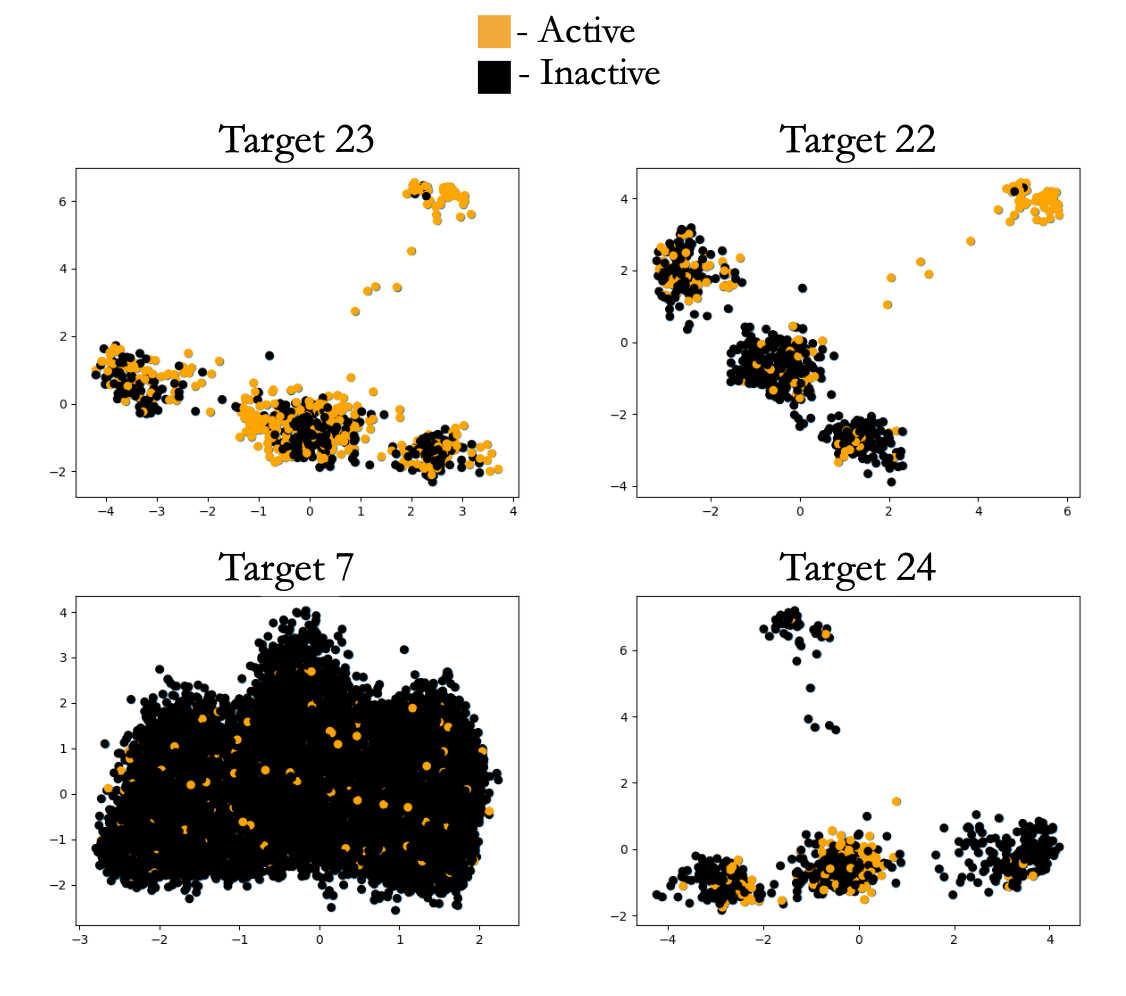
\includegraphics[width=.95\linewidth]{PCA.png}    \caption{
        PCA Dimension reduction for bioassay targets 23, 22, 7, and 24 
    }
    \label{fig:first-page}
\end{figure}

For bioassays 22 and 23, where the GNN strongly outperforms the NN, the active molecules are seen clustered together in the PCA plot. This indicates a strong structure-to-property relationship for those molecules, suggesting that the GNN’s ability to capture complex molecular relationships helped it identify the active molecules more accurately. The clustering implies that the active molecules share similar structural features, which the GNN can leverage to make more precise predictions.
In contrast, for bioassay 23, where the metrics for the NN and the GNN are very similar, it is observed that while there are distinct clusters of molecules, the active molecules are spread throughout each cluster. This suggests that there is no strong structure-to-property relationship for this bioassay, making it harder for both models to clearly distinguish between active and inactive molecules. 

When examining bioassay 7, where the NN outperformed the GNN on all betas except 3, it is apparent that there are no distinct clusters of molecules in the PCA plot. The molecules positive for that bioassay are fairly evenly distributed throughout the space, indicating that the structure-to-property relationship is weak or less clear for this bioassay. This lack of structure made it more challenging for the GNN to identify active molecules, explaining why the NN performed better at lower beta levels. However, at higher beta levels, the GNN’s better recall allowed it to catch more of the positives, which explains its slight edge at the beta level of 3.

From this PCA analysis, we can conclude that GNNs excel at identifying the structural trends that predict bioactivity, while NNs are more effective at recognizing the subtle trends that contribute to bioactivity. 

\subsection{Discussion}

This research is important as it aids in creating safer materials and product manufacturing by providing an approach to predict the bioactivity of PFAS molecules, which are of significant concern due to their environmental persistence and potential health impacts. By building a baseline of knowledge, this study helps researchers select the most effective approach for bioactivity prediction in their own work, suggesting neural networks (NNs) when minimizing false positives is critical and graph neural networks (GNNs) when maximizing recall and identifying active molecules is the priority.

These machine learning models can be used to screen for potentially safe PFAS compounds, allowing for a more efficient identification process to identify substances with minimal bioactivity to reduce environmental risks. This framework can serve as a first step in screening to identify promising compounds that warrant further, more extensive experimental testing to determine their safety.

However, there are limitations to consider. One key challenge in applying machine learning to structure to property prediction is the issue of class imbalances. The overrepresentation of inactive compounds compared to active ones can lead to biased model performance, as demonstrated by this research. This imbalance can result in models being more likely to predict active molecules as negative. This issue can be addressed through improved data collection, specifically for this research, aimed at building the PFAS database. Additionally, the concept known as activity cliff poses a difficult hurdle to surpass in structure to property prediction. The activity cliff is when a pair of compounds with high structural similarity have high property differences. This concept makes it very challenging for bioassay targets to be correctly predicted at a high level \textcite{Activity}. However, this should not rule out the use of machine learning as the approach still offers significant potential. While these models may not always predict bioactivity with perfect accuracy, they can still be valuable tools for narrowing down potential candidates that warrant further experimental investigation. 

\section{Ethical Considerations}

While my project aims at predicting bioactivity in PFAS molecules using machine learning, several ethical considerations must be addressed to ensure its responsible application. The primary concerns are related to bias, diversity, and the potential for contributing to inequalities. 

\subsection{Bias}

One significant ethical challenge is the potential for bias in machine learning models. These models are trained on data that may be incomplete or unrepresentative of the broader population. In the case of PFAS molecules, certain chemical structures or properties may be underrepresented in the data, particularly those found in molecules more prevalent in poorer countries. Wealthier countries tend to have more resources for testing and cataloging chemical compounds, leading to a larger and more diverse dataset for those molecules. In contrast, poorer countries may lack the funding and infrastructure to test and document a wide range of molecules, causing those compounds to be underrepresented in the training data. This disparity can result in the model misclassifying molecules that are more common in low-income regions. Such biases could have significant real-world consequences, particularly in regulatory decisions that may overlook or misjudge molecules with potential risks in these areas, exacerbating health and environmental inequities.

\subsection{Diversity of Data}

Another ethical consideration is ensuring the diversity of the data. If the dataset is limited to only molecules that are commonly studied or are easier to synthesize. This could result in a model that performs well for some molecules while performing poorly on others that may be less understood but equally critical from a health and environment standpoint. A careful review of the diversity of the data is essential in future iterations. 

\subsection{Potential Societal Impacts}

My project could have significant societal implications, particularly regarding the widespread contamination of PFAS molecules. PFAS compounds are highly persistent in the environment, making them a serious environmental concern. While the model may accurately predict bioactivity, helping identify harmful PFAS molecules, it could inadvertently encourage manufacturers to increase the use of PFAS in their products. Manufacturers might rely on the model to identify non-bioactive PFAS molecules, opting for these compounds rather than seeking safer alternatives when they are uncertain about bioactivity. This could lead to even greater environmental contamination, as the continued use of PFAS would exacerbate their persistence in ecosystems.

Additionally, access to the technology developed in my project could be uneven. Some researchers or manufacturers may lack the computational resources to replicate or build upon this research. Those with limited access may struggle to utilize these models for safer product development, potentially reinforcing existing inequalities in the ability to mitigate environmental harm, especially in underfunded countries or regions.




\appendix
\section{Replication Instructions}

All code and data for this project can be found at: https://github.com/wschwegler/Comps. To replicate this project, you need to install the following software and libraries:

\begin{itemize}
    \item \textbf{Python (At least version 3.8)}: Ensure that Python 3.8 or later is installed on your system. 
    
    \item \textbf{Anaconda}: It is highly recommended to use Anaconda to manage your Python environments and dependencies. 
    
    \item \textbf{PyCharm}: PyCharm was the IDE that this project was developed in; however, any IDE will suffice. You can download PyCharm from the official website: \url{https://www.jetbrains.com/pycharm/}.
    
    \item \textbf{Required Python Libraries}: The following Python libraries are required to run the project:
    \begin{itemize}
        \item \texttt{numpy}
        \item \texttt{pandas}
        \item \texttt{rdkit}
        \item \texttt{scikit-learn}
        \item \texttt{matplotlib}
    \end{itemize}
    
    \item \textbf{Graphite (for implementing the GNN)}: To install Graphite, clone this repository: https://github.com/LLNL/graphite

    After you have cloned the repository run this command:
    \begin{verbatim}
    pip install /filepath/graphite
    \end{verbatim}
\end{itemize}

\section{Code Architecture Overview}

The code architecture of this project is designed to be modular and easy to extend. Below is an overview of the main components and how they interact:

\begin{itemize}
    \item \textbf{Data Preparation}: 
    The data preparation for the GNN is handled in the file titled data set gen v2.py, where data is loaded, processed, and transformed into the appropriate format for the model. This includes converting SMILES strings to molecular fingerprints, creating feature arrays, and handling the target variables. The NN data preparation is handled in the NN file. 
    
    \item \textbf{Model Implementation}: 
    The core machine learning models used for the project are implemented in the files titled NN and GNN. The NN file handles the data processing, model training, and classification report generation. The GNN file just contains the model and the data processing and classification report generation are handled in separate files

    \item \textbf{PCA}: 
    The file titled PCA performs PCA dimension reduction on the binary fingerprint data and visualizes it. 

    \item \textbf{Model Evaluation and Metrics}: 
    The file titled GNN Eval is utilized to load model checkpoints and generate classification reports. The file titled f1 is utilized to calculate the f-beta scores. 

\end{itemize}



\printbibliography
\end{document}
